\documentclass{article}
\usepackage{listings}
\usepackage{lipsum} % pentru generarea de texte de umplere
\usepackage{graphicx}
\usepackage{caption}
\usepackage{enumitem}
\usepackage{hyperref}
\usepackage{tikz}
\usetikzlibrary{shapes,arrows}

\title{Proiect Arduino - Sistem de Monitorizare și Avertizare}
\author{Alin-Ioan Alexandru 322CA}
\date{}
\begin{document}

\maketitle

\section{Introducere}
Proiectul Arduino implementează un sistem de monitorizare și avertizare utilizând un senzor ultrasonic de distanta, un microcontroller Arduino Uno și doi actuatori, un LED si un buzzer pentru a indica anumite condiții. Scenariul practic imaginează utilizarea a doi senzori ultrasonici de distanta.

\section{Scenariu Practic}
Un robot sau chiar un vehicul autonom are nevoie are nevoie de mai mulți senzori atât pentru a determina poziția sa, cât și distanța față de alte obiecte. Acest proiect își propune să simuleze o versiune simplificată a unui sistem de senzori pentru a avertiza ”robotul” în cazul în care distanța se aproprie de un prag limită.

\section{Schema bloc}

\begin{figure}[h]
    \centering
    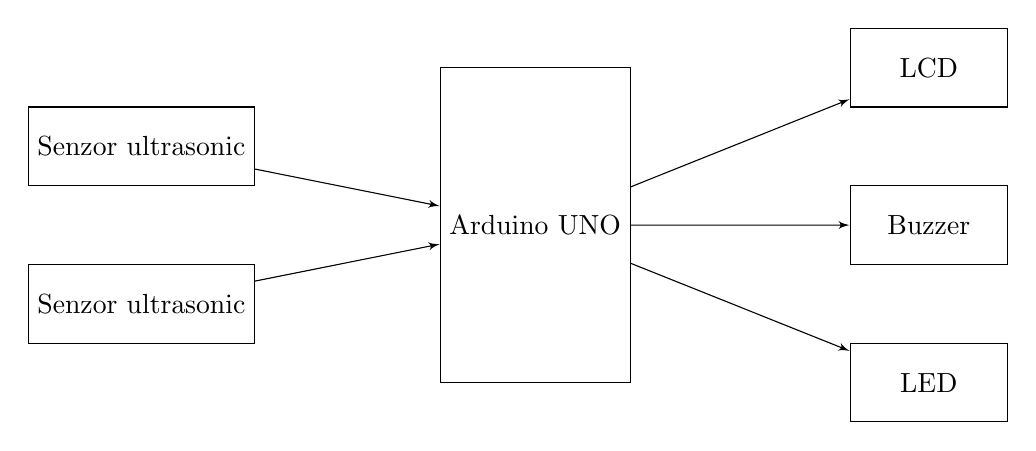
\begin{tikzpicture}[auto, node distance=1cm,>=latex']
  
      % Componente inițiale
      \node [draw, rectangle, node distance=4cm, minimum height=1cm] (componenta1) {Senzor ultrasonic};
      \node [draw, rectangle, below of=componenta1, node distance=2cm, minimum height=1cm] (componenta2) {Senzor ultrasonic};
  
      % Componenta mare
      \node [draw, rectangle, right of=componenta1, minimum height=4cm, node distance=5cm, yshift=-1cm] (componenta_mare) {Arduino UNO};
  
      % Componente mici
      \node [draw, rectangle, right of=componenta_mare, minimum width=2cm, minimum height=1cm, node distance=5cm, yshift=2cm] (componenta3) {LCD};
      \node [draw, rectangle, below of=componenta3, minimum width=2cm, minimum height=1cm, node distance=3cm, yshift=1cm] (componenta4) {Buzzer};
      \node [draw, rectangle, below of=componenta4, minimum width=2cm, minimum height=1cm, , node distance=3cm, yshift=1cm] (componenta5) {LED};
  
      % Linii de legatura
      \draw [->] (componenta1) -- (componenta_mare);
      \draw [->] (componenta2) -- (componenta_mare);
      \draw [->] (componenta_mare) -- (componenta3);
      \draw [->] (componenta_mare) -- (componenta4);
      \draw [->] (componenta_mare) -- (componenta5);
  
    \end{tikzpicture}
    \caption{Schemă bloc}
  \end{figure}

\section{Circuitul}

\begin{figure}[h]
    \centering
    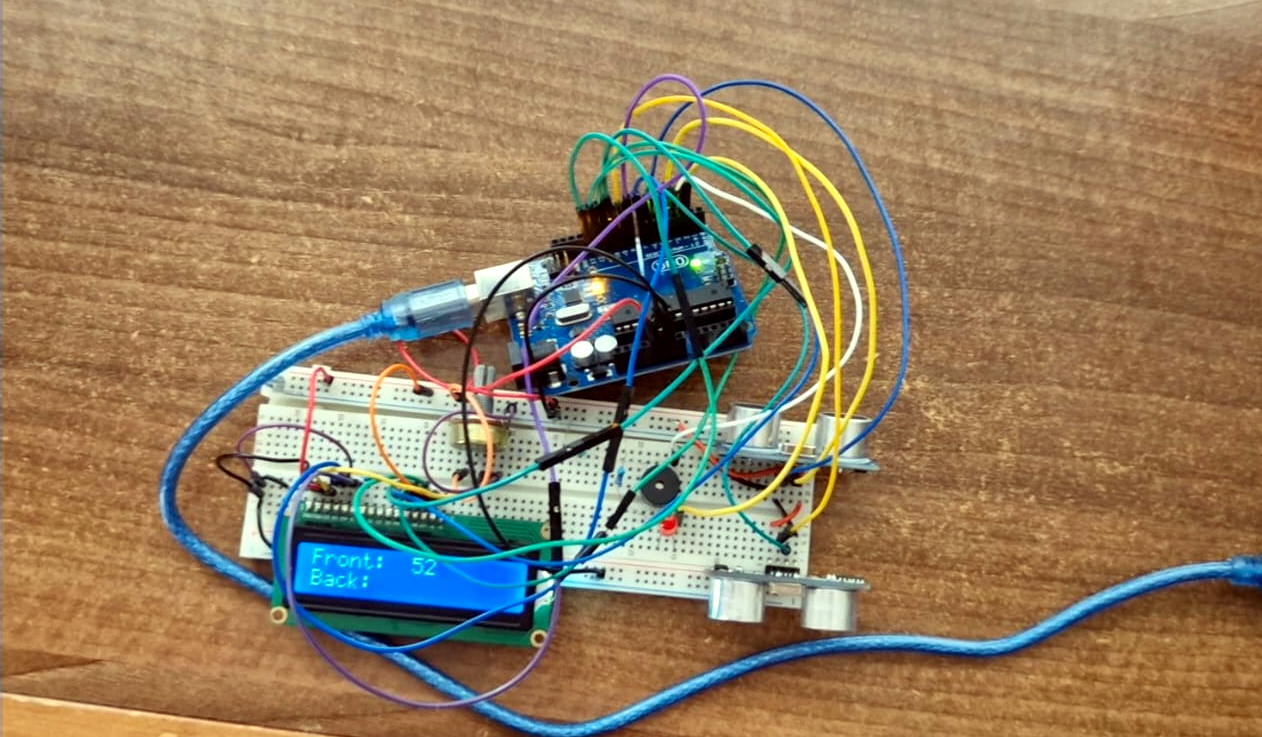
\includegraphics[width=0.8\textwidth]{circuit.jpeg}
    \caption{Circuitul}
\end{figure}

\begin{itemize}
    \item \textbf{Senzori ultrasonici:} Măsoară distanța în fața și în spatele breadboard-uilui și transmit aceaste valoari către Arduin. Acestia sunt conectați la sursa de 5V din Arduino și la GND. Pinul Trig este cel prin care se primeste semanlul care generează undele sonore, iar pinul Echo este cel prin care se trimite durata măsurătorii către Arduino.
    \item \textbf{Arduino Uno:} Microcontrollerul preia datele de la senzori și compară valoarea cu pragurile stabilite. În funcție de rezultat, controlează LED-ul si buzzerul pentru a avertiza că un corp este la o distanța mult prea apropriată.
    \item \textbf{LED și Buzzer:} Actuatori care se activează atunci când un cropul se aproprie mult prea mult de circuit. LED-ul este conectat la pinul 2 al zonei digitale de pe Arduino, iar buzzerul la pinul 3, deoarece are nevoie de PWM. Ambele componenete au în serie câte un rezistor care se duce către GND.
    \item \textbf{LCD:} Primește distanțele calculate de Arduino și le afișează pentru fiecare senzor. Dispune de un potețiometru folosit pentru a regla contrastul ecranului.
\end{itemize}

Modul de funcționare a fost prezentat la curs.
\pagebreak

\section{Bill of materials}

\begin{itemize}
    \item \href{https://www.optimusdigital.ro/ro/senzori-senzori-ultrasonici/9-senzor-ultrasonic-hc-sr04-.html}{Senzor ultrasonic HC-SR04} x 2
    \item \href{https://www.optimusdigital.ro/ro/placi-avr/4561-placa-de-dezvoltare-compatibila-cu-arduino-uno-r3-atmega328p-atmega16u2-cablu-50-cm.html?search_query=arduino+uno&results=136}{Placa de Dezvoltare Compatibila cu Arduino UNO R3}
    \item \href{https://www.optimusdigital.ro/ro/audio-buzzere/634-buzzer-pasiv-de-5-v.html?search_query=buzzer&results=59}{Buzzer Pasiv de 5 V}
    \item \href{https://www.optimusdigital.ro/ro/optoelectronice-led-uri/696-led-rou-de-3-mm-cu-lentile-difuze.html?search_query=LED&results=782}{LED Roșu de 3 mm cu Lentile Difuze}
    \item \href{https://www.optimusdigital.ro/ro/optoelectronice-lcd-uri/867-modul-lcd-1602-cu-backlight-galben-verde-de-5v.html?search_query=lcd&results=202}{Modul LCD 1602}
    \item \href{https://www.optimusdigital.ro/ro/prototipare-breadboard-uri/8-breadboard-830-points.html?search_query=breadboard&results=141}{Breadboard}
    \item Fire de legătură.
    \item Rezistori x 3
\end{itemize}

\end{document}